\section{Vorwort zu den Simulationen} \label{sec:vorwort}
Die in den folgenden Abschnitten verwendeten Daten der einzelnen Elemente für Dichten, Absorptionskanten und Fluoreszenzlinien enstammen, außer anders erwähnt, der kostenlosen Software Hephaestus. Hephaestus ist Teil des Softwarepakets Demeter, welches von Bruce Ravel entwickelt und unter \textit{\url{https://bruceravel.github.io/demeter/}} erreichbar ist. \newline
Die Berechnungen der Transmissionssignale geschieht mit Hilfe eines Online-Tools des CXRO (center of x-ray optics). Entwickelt von Eric Gullikson und im Netz unter \textit{\url{http://henke.lbl.gov/optical_constants/}} aufrufbar.\newline

Die Herstellung der Proben zur Validierung am Synchrotron übernimmt Christine Gottschalk aus der AG Vogt, TU Freiberg. Dafür werden hoch- und niederviskose Glanzlacke verwendet. Dieses Lackgemisch bildet das Grundgerüst aller verwendeten Schichten. Weitere, schwerere Elemente werden im Herstellungsvorgang nur zugemischt. Hinzugegeben werden außerdem ein Entschäumer, ein Oberflächenadditiv und ein Dispergieradditiv. Als Substrat dient eine Polyesterfolie. Die exakte elementare Zusammensetzung ist nicht bekannt und wird als $C_{16}H_{14}O_{3}$ abgeschätzt. Die Dichte des Lacks wurde durch Wiegung auf etwa \SI{0.87}{\gram\per\cubic\centi\meter} bestimmt \cite{christine}. Als Träger dient ein Siliziumnitridfenster $Si_{3}N_{4}$ der Stärke \SI{200}{\nano\meter}. Das Probendesign versucht sich in Bezug auf die Massenanteile der beigemischten schwereren Elementen und in Bezug auf die verwendeten Elemente an den Möglichkeiten der Kooperationspartner zu orientieren.\newline

Damit die Detektoreffekte im realen Experiment auch sichtbar sind, ist es notwendig, dass die Effekte, welche bei der Simulation visualisiert werden, signifikant sind. Dies ist besonders wichtig, da bei der Durchführung am Synchrotron die in \cref{modell} genannten Quellen für Unschärfe hinzukommen. Daher ist die Zielsetzung dieser Simulationen, dass sowohl hinreichend viele Detektorsignale vorhanden sind, als auch dass an der zu untersuchenden Kante die Intensität um mindestens 10\% innerhalb der Struktur abfällt. Andererseits soll mit Hinblick auf eine potentielle Untersuchung mit Transmissionsspektroskopie die Probe, wenn möglich, so entworfen werden, dass zumindest eine schwache Restintensität hinter der Probe detektiert werden kann.\newline

Absorptionseffekte in höher liegenden Schichten bieten dafür die grundlegenden Bedingungen. Dabei unterscheiden sich die von den Detektoren registrierten Intensitäten (Anm.: bei Betrachtung der Sekundärfluoreszenz könnten auch andere Elemente detektiert werden) je nach chemischer Komposition und Dichte der Schicht, die die Fluoreszenzstrahlung auf ihrem Weg zum Detektor passieren muss. Wenn nicht anders erwähnt sind die Proben so entworfen, dass der Absorptionsweg der Fluoreszenz bei Anregung an einer Schichtgrenze nur durch eine Schicht dieser Ebene führt wie nachfolgend in \cref{fig:strahlengang} illustriert ist.  
\begin{figure}[H] 
  \centering
     \includegraphics[width=0.9\textwidth]{illustrations/durchzelle.png}
  \caption[Minimalistischer Schnitt durch Probe und Detektor]{Minimalistischer Schnitt durch Probe und Detektor in dem die wichtigsten geometrischen Größen abgebildet sind:  Vom anregenden Strahl (zentral) ausgehend sind die Winkel $\alpha$ und $\beta$ aufgetragen welche die innere $r_i$ und äußere $r_a$ aktive Detektorfläche sowie die Wege durch die oberste Schicht $c_i$ und $c_a$ aufspannen. $d_{opt}$ ist der Höhenunterschied zwischen Probenoberfläche und Detektor, $h$ die Dicke der obersten Schicht. Durch $\beta$ und $h$ ergibt sich die Gesamtbreite der Zelle zu $r_p$.}
  \label{fig:strahlengang}
\end{figure}
Der Probe-Detektor-Abstand wird mit $d_{opt}=\SI{2.43}{\milli\meter}$ als ideal angenommen. Daraus resultiert nach \cref{beta} der äußere Öffnungswinkel zu $\beta = \SI{54.9}{\degree}$, nach \cref{alpha1} ergibt sich der innere Öffnungswinkel zu $\alpha = \SI{36.9}{\degree}$ . Dies gewährleistet, dass die Absorption der Fluoreszenzstrahlung nur in einer Schicht stattfindet, insofern zwischen den Schichten angeregt wird und die Schichten in dieser Ebene gleich hoch sind. Für die Betrachtung des Absorptionswegs $c_a$ unter $\beta$ durch die Probe ergeben sich für die Probenbreite $r_{p}$, die Probenhöhe $h$ und den kürzeren Absorptionsweg $c_i$ die nachfolgenden Gleichungen.

\begin{alignat}{2}	
r_{p} &= c_a \cdot \sin(\SI{54.9}{\degree}) &= 0.82 \cdot c_a \label{eq:rp}	\\[10pt]
h &= c_a \cdot \cos(\SI{54.9}{\degree}) &= 0.57 \cdot c_a \label{eq:h} \\[7pt]		
c_i &= c_a \cdot \frac{\cos(\SI{54.9}{\degree})}{\cos(\SI{36.9}{\degree})} &= 0.72 \cdot c_a \label{eq:ci}
\end{alignat}

Im Rahmen dieser Arbeit müssen nicht alle Simulationsparameter variiert werden, nachfolgend sind einige erörtert. Da die Anregungsintensität je nach Energie und Beamline stark schwankt und diese qualitativ keine Auswirkung in der Simulation besitzt, wird sie auf \SI{e9}{Photonen\per\second} festgelegt. Weiterhin wird die Schrittweite in x-Richtung auf \SI{500}{\nano\meter} gesetzt, da dies in der Größenordnung der Spotausdehnung am Synchrotron liegt. Vergangene Untersuchungen liefern für die z-Schrittweite \SI{500}{\nano\meter} als guten Kompromiss zwischen Simulationsgeschwindigkeit und -qualität bei genügend großen Probenstrukturen. Mit gleicher Begründung werden die betrachteten Raumwinkel in 15 Segmente und die Detektorradien in 20 Abschnitte aufgeteilt. Wenn nicht ausdrücklich anders erwähnt sind die späteren Simulationen mit eben genannten Parametern ausgeführt worden.\newline

Ausdrückliche Zielsetzung der Simulationen ist es einen signifikanten Kontrast in den von den Detektorsegmenten gemessenen Intensitäten der Fluoreszenzsignale zu erreichen. Ausgehend von einem Anregungspunkt heißt das, dass die detektierten Fluoreszenzphotonen unter den möglichen Raumrichtungen unterschiedlich stark absorbierende Schichten passieren müssen. Dies gelingt durch Variation von Schichtdicken und -breiten von zwei alternierenden, verschieden stark absorbierenden Schichten.